\section{OOP PRINCIPLES REVISITED}

La OOP è un paradigma di programmazione basato sul concetto di oggetto. Questo oggetto contiene dati e/o metodi/procedure. La caratteristica maggiore è che il paradigma oop le procedure degli oggetti possono accedere ai dati.


\subsection{Oggetto}

\begin{itemize}
\item è un istanza della classe;
\item definizione secondo Grady Booch: "un oggetto rappresenta un articolo (item), un'unità o un'entità individuale, identificabile, reale o astratta che sia, con un ruolo ben definito nel dominio del problema e un confine altrettanto ben stabilito";

Generalmente un oggetto è caratterizzato da uno stato, da un comportamento e da un'identità, come bene simboleggiato da questa illustrazione tratta, come quelle che seguono, da G. Booch, Object-oriented Analysis and Design:

\begin{figure}[H]
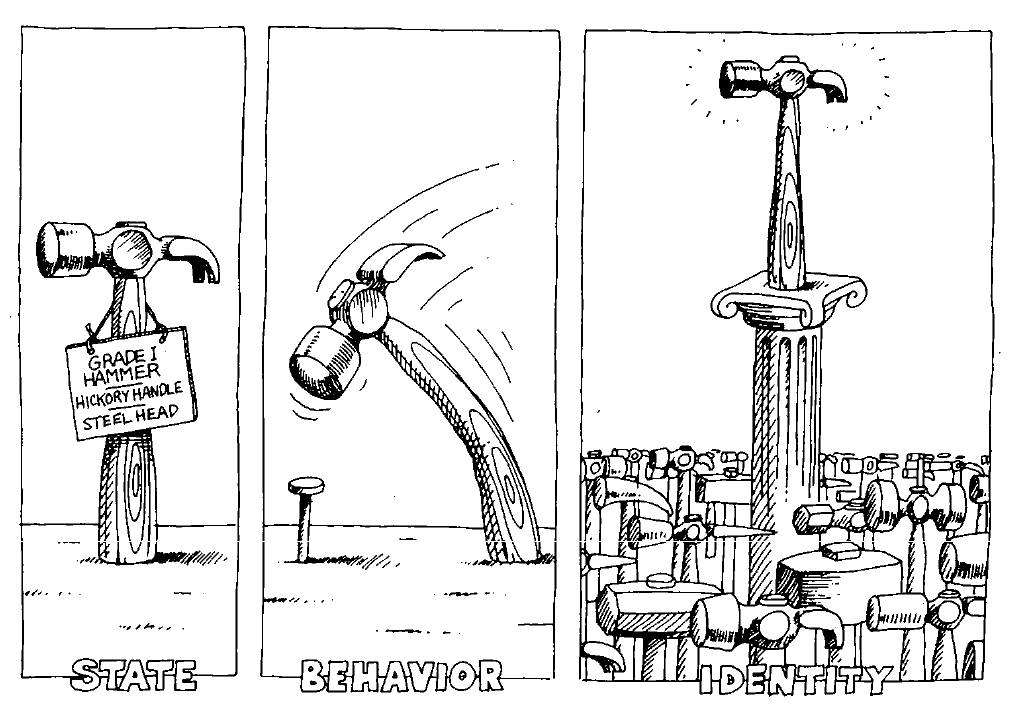
\includegraphics[scale=0.4]{images/oggetto}
\caption{Definizione di oggetto  \label{fig:oggetto}}
\end{figure}
\end{itemize} 

\subsubsection{Elementi fondamentali di un oggetto}

“Un oggetto possiede stato, comportamento e identità; la struttura e il comportamento di oggetti simili sono definiti nella loro classe comune; i termini di istanza e oggetto sono intercambiabili.” [Grady Booch].

\paragraph{Stato}

Gli oggetti, tipicamente, non vengono creati per permanere in un determinato stato; al contrario, durante il loro ciclo di vita transitano in una serie di fasi.

Tipi di stato:
\begin{itemize}
\item \textbf{oggetto con un insieme finito di stati}: per esempio l'oggetto lampadina ha 2 stati: acceso e spento. Un altro esempio è una lampadina evoluta con un numero ben definito di diverse intensità di luce, quindi avrò gli stati spenta, accesa intensità 1, accesa intensità 2, ..., accesa intensità max;

\item \textbf{oggetto con un numero di stati non numerabili}: per esempio un sistema di illuminazione delle stanze la cui funzione sia accendere/spegnere i vari faretti in funzione del numero di persone presenti nelle stanze. Sebbene questo numero sia delimitato (il numero massimo di persone stipabili all'interno della stanza), non è conveniente indicare i vari stati dell'oggetto (una persona, due persone, tre persone, …);

\item \textbf{oggetto con stati teoricamente infinito}: per esempio, si consideri un'estensione del sistema precedente, in cui la decisione di accendere e/o spegnere l'illuminazione dipenda anche dal valore dell'intensità luminosa segnalata da un apposito oggetto (sensore). In questo caso, il dominio dei valori dei dati forniti sarebbe teoricamente infinito.

\end{itemize}

Lo stato di un oggetto è molto importante poiché ne influenza il comportamento futuro. Gli oggetti, almeno loro, hanno una certa memoria storica. Tipicamente, sottoponendo opportuni stimoli a un oggetto (invocazione dei metodi, o invio di messaggi se si preferisce), questo tende a reagire, nella maggior parte dei casi, in funzione del suo stato interno.

\textbf{Esempio 1}: se una sua istanza si trova nello stato di accesa e ne viene richiesta nuovamente l'accensione (turnOn()), nulla accade.

\textbf{Esempio 2}: se si preme il tasto di play senza aver inserito un CD, nulla accade (viene generata un'eccezione), mentre la pressione dello stesso tasto, con CD inserito, avvia il suono della musica.

Lo stato di un oggetto è un concetto dinamico e, in un preciso istante di tempo, è dato dal valore di tutti i suoi attributi e dalle relazioni instaurate con altri oggetti (che alla fine sono ancora particolari valori, indirizzi di memoria, attribuiti a specifici attributi).

È molto importante nascondere quando possibile lo stato di un oggetto al resto del mondo. Sicuramente deve esserne sempre nascosta l'implementazione (principio \textit{dell'information hiding}) e quando possibile anche lo stato stesso (minimizzare l'accoppiamento di tipo).

\paragraph{Comportamento}

Una volta studiato e formalizzato lo stato di un oggetto si è effettuato un passo in avanti nel processo di astrazione.

Tipicamente un oggetto interagisce con altri scambiando messaggi, ossia rispondendo agli stimoli provenienti da altri oggetti (richiesta di un servizio) e, a sua volta, inviandoli ad altri al fine di ottenere la fornitura di "sottoservizi" necessari per l'espletamento(completamento) del proprio. Quindi, il comportamento di un oggetto è costituito dalle sue operazioni visibili e verificabili dall'esterno.

"Il comportamento stabilisce come un oggetto agisce e reagisce, in termini di cambiamento del proprio stato e del transito dei messaggi." [Booch].

\textbf{Un'operazione} è una qualsiasi azione che un oggetto è in grado di richiedere a un altro al fine di ottenere la reazione desiderata.

È evidente che la relazione esistente tra stato di un oggetto e comportamento è di mutua dipendenza: è possibile considerare "lo stato di un oggetto, in un certo istante di tempo, come l'accumulazione dei risultati prodotti dal relativo comportamento", il quale, a sua volta, dipende dallo stato in cui si trovava l'oggetto all'atto dell'esecuzione del "comportamento".

\paragraph{Identità}

 \noindent L'identità di un oggetto è la caratteristica che lo contraddistingue da tutti gli altri. Spesso ciò è dato da un valore univoco. Per esempio un oggetto ContoCorrente è identificato dal relativo codice, da una persona, dal codice fiscale, e così via.

 \subsection{Classe}
 \begin{itemize}
\item è un prototipo che descrive com'è fatto una certa tipologia di oggetti.
 \end{itemize}
 
 \subsection{Tempo di implementazione vs tempo di esecuzione}
  \begin{figure}[H]
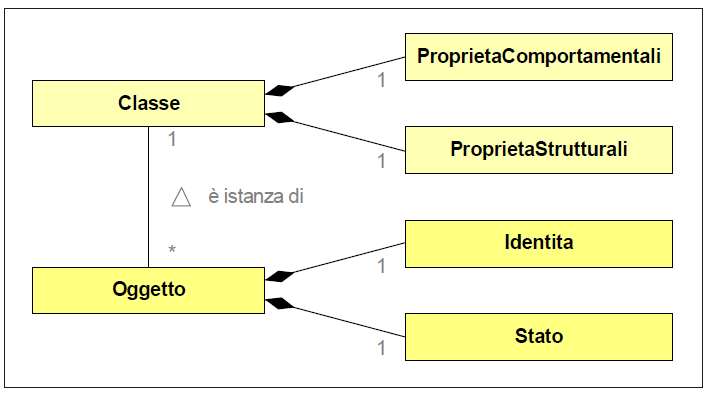
\includegraphics[scale=0.7]{images/esecuzioneVSimplementazione}
\caption{\textit{In questo (meta) modello sono distinte più nettamente le caratteristiche a tempo di implementazione (Classe, ProprietàComportamentali e ProprietàStrutturali) da quelle a tempo di esecuzione (Oggetto, Identità e Stato). \textbf{Le proprietà comportamentali} rappresentano l'insieme dei metodi esposti da una classe e quindi invocabili da parte di oggetti istanze di altre classi, mentre quelle \textbf{strutturali} rappresentano l'insieme degli attributi. Per quanto concerne la notazione, per il momento si consideri il diamante pieno (relazione di composizione) come una relazione strutturale molto forte tra due entità, di cui le istanze della classe con il diamante rappresentano il concetto generale costituito dalle istanze delle altre classi associate.}\label{fig:ered0}}
\end{figure}

\subsection{Principi cardini della OOP}

\subsubsection{Incapsulamento (information hiding)}
L'incapsulamento è il meccanismo che rende possibile il famoso principio dell'information hiding (nascondere le informazioni). Con tale termine ci si riferisce alla capacità degli oggetti di mostrare al mondo esterno, la propria organizzazione in termini di struttura e logica interna.

Una delle motivazioni alla base \textbf{dell'information hiding} è data dalla necessità di creare uno strato di separazione tra gli oggetti clienti e quelli fornitori. In altre parole è necessario separare l'interfaccia propria di un oggetto dalla sua implementazione interna. In sostanza l'interfaccia (anche se implicita) rappresenta il contratto stipulato tra gli oggetti client e quelli server. Ciò è vantaggioso al fine di aumentare il riutilizzo del codice e di limitare gli effetti generati dalla variazione della struttura di un oggetto.

In genere \textbf{l'incapsulamento standard} prevede che le classi non abbiano alcuna conoscenza della struttura interna delle altre, e in particolare di quelle di cui possiedono un riferimento, con la sola eccezione della firma dei metodi esposti nella relativa interfaccia. Ciò permette a ogni classe di modificare, aggiungere, rimuovere parte del proprio comportamento e della propria struttura interna senza generare alcun effetto sulle restanti classi.

Questo è vero fintantoché le variazioni non abbiano come dominio metodi appartenenti all'interfaccia della classe: è sufficiente anche la variazione di un solo parametro della firma di un metodo dell'interfaccia per rendere necessaria la modifica delle classi client.

Il principio dell'incapsulamento standard, in Object Oriented, si realizza rendendo privata la struttura interna della classe. Chiaramente una classe con tutti i metodi e gli attributi privati sarebbe di ben poco utilizzo.

Ciò che si desidera è, in definitiva, conferire una visibilità privata a quanta più parte di struttura e comportamento possibile (soprattutto agli attributi), limitandosi a esporre specifici metodi.
\paragraph{Difetti dell'incapsulamento}

Il nascondere il più possibile l'organizzazione della struttura delle classi, di fatto, limita o addirittura inibisce l'ereditarietà. Metodi e attributi privati non sono ereditati automaticamente, o meglio, sono ancora ereditati ma non accessibili, e quindi ridefinibili, dalla classe ereditante. In estrema sintesi si può asserire che la privacy non aiuta l'ereditarietà.

    \begin{itemize}
    \item Esempio di incapsulamento [Java] :
    \begin{lstlisting}
public class cubo
{
    // Dichiarazione delle proprieta: si noti che sono definite tutte private.
    private int lunghezza;
    private int larghezza;
    private int altezza;
    // Metodi "Mutator" per la modifica delle proprieta
    public void setLunghezza(int lun)
    {
        lunghezza = lun;
    }
    public void setLarghezza(int lar)
    {
        larghezza = lar;
    }
    public void setAltezza(int alt)
    {
        altezza = alt;
    }
    // Metodi "Accessor" per ricavare i valori delle proprieta
    public int getLunghezza()
    {
        return lunghezza;
    }
    public int getLarghezza()
    {
        return larghezza;
    }
    public int getAltezza()
    {
        return altezza;
    }
    // Metodo pubblico che visualizza il volume del cubo, usando le proprieta
    // interne della classe
    public void visualizzaVolume()
    {
        System.out.println(lunghezza * larghezza * altezza);
    }
}    \end{lstlisting}
     \end{itemize}


\subsubsection{Ereditarietà}

Si tratta di un meccanismo attraverso il quale un'entità più specifica incorpora struttura e comportamento definiti da entità più generali. Questo significa che la sottoclasse possiede tutti i campi e metodi della superclasse. Il fine cui si dovrebbe tendere attraverso l'utilizzo dell'ereditarietà è il "riutilizzo del tipo" perchè non c'è bisogno di ridescrivere quanto viene ereditato. Viceversa, le modifiche apportate alla sottoclasse sono limitate solo ad essa e non si applicano alla superclasse.

È possibile pensare all'ereditarietà come a un meccanismo in grado di prendere un elemento di partenza, clonarlo e di modificare e/o aggiungervi struttura e comportamento ulteriori.

\begin{figure}[H]
\includegraphics[scale=0.8]{images/ereditarietàUML}
\caption{\textit{La relazione di generalizzazione tra due classi è mostrata in UML attraverso una freccia collegante l'elemento figlio al proprio genitore, con un triangolo vuoto posto in prossimità di quest'ultimo.} \label{fig:oggetto}}
\end{figure}

\paragraph{Difetti}
\begin{itemize}
\item l’ereditarietà presenta punti di contrasto con il principio dell’incapsulamento: la classe antenata deve esporre propri dettagli interni alla classe ereditante, quindi modifiche alle classi antenate tendono a ripercuotersi su quelle discendenti.
\end{itemize}

\paragraph{Pregi}
\begin{itemize}
\item riutilizzo del codice, perchè il comportamento comune è definito una sla volta nella classe madre e riutilizzato nelle classi discendenti;
\item semplificazione della modellazione di sistemi reali;
\item utilizzo del polimorfismo perchè permette di dichiarare per una stessa operazione (metodo) definita in una classe antenata, diverse implementazioni ognuna localizzata in una delle classi discendenti;
\end{itemize}

\paragraph{Principio della sostituibilità}
Un’istanza di una classe discendente può sempre essere utilizzata in ogni posto ove è prevista un’istanza di una classe antenata.

\paragraph{Applicazione parziale del pattern Command}

\begin{figure}[H]
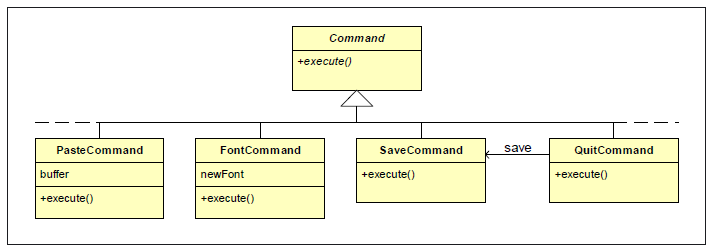
\includegraphics[scale=0.8]{images/commandEreditarita}
\caption{\textit{Gang Of Four (BIB04)} \label{fig:ered1}}
\end{figure}
In questo modello si è voluto mostrare un utilizzo più operativo della relazione di eredità. Come si può notare è possibile definire una classe generica Commanddotata di un metodo astratto execute()e quindi tutta una serie di specializzazioni atte a definire il comportamento del metodo in funzione delle responsabilità dello specifico comando. Per esempio, nella classe PasteCommand, il metodo execute() si occupa di copiare quanto presente nel buffer nell’area selezionata; nella classe QuitCommand, il metodo ha l’incarico di terminare l’esecuzione del programma (eventualmente chiedendo conferma) e, nel caso in cui vi siano cambiamenti non ancora memorizzati, ha l’ulteriore responsabilità di richiedere se salvare o meno i cambiamenti prima di terminare l’esecuzione.


\paragraph{Quando non applicare l'ereditarità}
\begin{itemize}
\item qualora in una struttura gerarchica un oggetto possa “trasmutare”, evidentemente l’applicazione della relazione di estensione è inappropriata e quindi è opportuno ricorre alla composizione;
\item ogniqualvolta in una struttura gerarchica un oggetto possa appartenere a più “tipi”, nuovamente non è opportuno utilizzare la relazione di generalizzazione.
\end{itemize}

\begin{figure}[H]
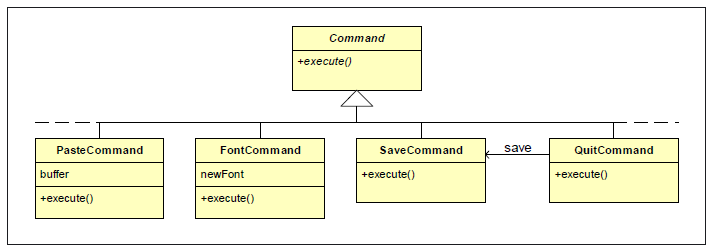
\includegraphics[scale=0.8]{images/commandEreditarita}
\caption{\textit{Esempio di errato utilizzo della relazione di ereditarietà. Da notare che con il termine di sviluppatore si intende far riferimento ai diversi ruoli implicati nella costruzione di sistemi (architetti, programmatori, tester, ecc.)} \label{fig:ered2}}
\end{figure}

È possibile identificare una serie di oggetti che esibiscono segmenti comuni di comportamento e/o struttura (per esempio la classe Persona) al quale ognuno aggiunge ulteriori specializzazioni (Cliente, Manager, Contabile, ecc.).

Cosa accade se un Commerciale, a un certo punto del suo ciclo di vita decide di diventare uno Sviluppatore? sarebbe necessario dar luogo a un’altra istanza, questa volta di tipo Sviluppatore, e quindi avere due oggetti diversi relativi allo stesso individuo con due identificatori distinti, con tutti i problemi derivanti. Ancora, cosa succederebbe se alcuni sviluppatori (per esempio Antonio Rotondi, Roberto Virgili), fossero così eccelsi da svolgere anche funzioni di Direttore? Queste due semplici domande sono sufficienti a dimostrare tutti i limiti dell’utilizzo della relazione di generalizzazione in contesti come questo.

\begin{figure}[H]
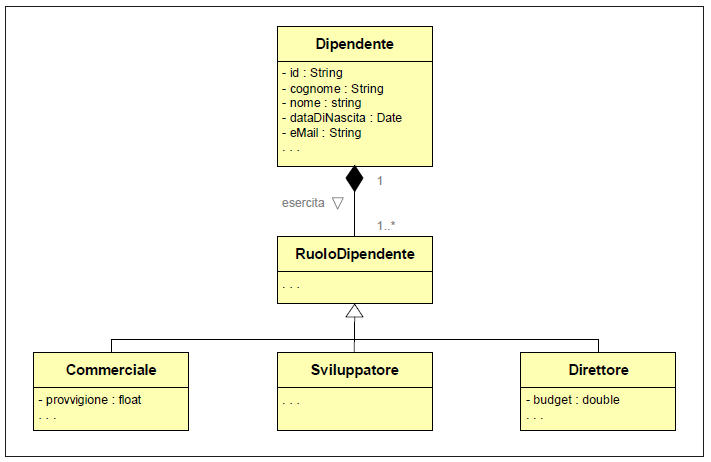
\includegraphics[scale=0.8]{images/ereditarietaOk}
\caption{\textit{Rappresentazione dei ruoli attraverso la relazione di composizione. Da notare che la classe RuoloDipendente non è strettamente necessaria} \label{fig:ered5}}
\end{figure}
\subsubsection{Polimorfismo}

Polimorfismo deriva dalle parole greche polys (= molto) e morphé (=forma): significa quindi “molte forme”. Si tratta di una caratteristica fondamentale dell'Object Oriented, relativa alla capacità di supportare operazioni con la medesima firma e comportamenti diversi, situate in classi diverse ma derivanti da una stessa antenata.

Per poter realizzare il polimorfismo, i linguaggi di programmazione devono realizzare meccanismi di collegamento dinamico (\textbf{dynamic binding}, detto anche late binding, ossia collegamento ritardato). Con ciò si fa riferimento alla capacità di associare l'invocazione di un metodo alla relativa implementazione presente in un oggetto in tempo di esecuzione.Il motivo è abbastanza evidente: l'istanza della classe che deve eseguire il metodo è conosciuta solo durante l'esecuzione del programma in quanto, in diversi periodi dell'esecuzione, la stessa invocazione potrebbe essere soddisfatta da oggetti appartenenti ad istanze di classi diverse (che ereditano da una stessa classe o che implementano una comune interfaccia).

In un'organizzazione gerarchica ottenuta per mezzo dell'ereditarietà, si effettua un \textbf{upcasting} ogniqualvolta un oggetto di una classe discendente viene trattato (casted) come se fosse un'istanza della classe progenitrice (ciò avviene in maniera implicita). Mentre, con il termine di \textbf{downcasting}, si intende l'operazione opposta, ossia si tenta di trattare un riferimento di un tipo antenato come un'istanza di uno specifico discendente.

\paragraph{Overloading e Overriding}

\subparagraph{Overriding}

Il termine overriding è intimamente legato al polimorfismo: quando in una classe discendente si ridefinisce l'implementazione di un metodo, in gergo si dice che se ne è effettuato l'overriding. In sostanza si crea una nuova definizione della funzione polimorfica nella classe discendente.


    \begin{itemize}
    \item Esempio di overriding in Java :
    \begin{lstlisting}
public class Dipendente{
	
  private String nome;
  private String cognome;
  private int oreLavorativeMensili;
  private int retribuzioneOraria;

  public int getOreLavorativeMensili(){
    return oreLavorativeMensili;
  }
    
  public int getRetribuzioneOraria(){
    return restribuzioneOraria;
  }

  public int stipendio(){
    return oreLavorativeMensili * retribuzioneOraria;
  }  
}
\end{lstlisting}

    \begin{lstlisting}
public class ResponsabileDiProgetto extends Dipendente {

  private int bonus;

  public int stipendio(){
    int stipendioBase=(getOreLavorativeMensili() * getRetribuzioneOraria());
    return stipendioBase + bonus;
  }
}
\end{lstlisting}
\end{itemize}


\subparagraph{Overloading}

Il termine overloading ha a che fare con la definizione di diversi metodi con nome uguale, ma firma diversa (non esattamente, visto che la variazione del solo tipo di ritorno non costituisce un overloading). Per l'utilizzo di questa tecnica non è necessario dar luogo a particolari legami di ereditarietà.


    \begin{itemize}
    \item Esempio di overload in Java :
    \begin{lstlisting}
public class OperazioniSuNumeri {
  public int somma(int x, int y) {
    return x+y;
  }

  public float somma(float x, float y) {
    return x-y;
  }
}
\end{lstlisting}
\item Dal punto di vista implementativo :
    \begin{lstlisting}
public class Implementazione {

  OperazioniSuNumeri numeri = new OperazioniSuNumeri();
  sommaInteri = numeri.somma(3,4);
  System.out.println("La somma tra interi e:");
  System.out.println(sommaInteri);

  sommaFloat = numeri.somma(2.1,8.3);
  System.out.println("La somma tra float e:");
  System.out.println(sommaFloat);
}
   \end{lstlisting}
     \end{itemize}

\subsection{Evoluzione della programmazione}

Il primo linguaggio ad oggetti è stato SmallTalk.

\textbf{Osservazione:} Nella programmazione ad oggetti ciò che conta in una classe non sono i dati, ma sono i messaggi. Messaggi e metodi sono la stessa cosa. Nel SmallTalk quando dicevo che l’oggetto A invia un messaggio all’oggetto B significa che l’oggetto A invoca un metodo su B.
Un oggetto o una classe dev’essere vista come un insieme di comportamenti non di dati. Chi usa la mia classe non deve fregarsene com’è fatta all’interno. L’unica cosa che a lui deve interessare sono i messaggi quindi il comportamento (behaviour o interfaccia) che la mia classe espone verso l’esterno.

\subsubsection{Interfaccia}
Insieme dei metodi pubblici di una classe. Che può essere fisica,reale quando qualcuno mi scrive direttamente “interface” in java o classe virtuale pura in c++, sia che sia implicita ovvero la lista dei suoi metodi pubblici.

\subsubsection{Perchè si è arrivati alla programmazione ad oggetti?}
Il problema parte dalla programmazione procedurale. Non possiamo dire che quest’ultima non sia utile, anzi, ogni cosa ha il suo caso d’uso. Non esiste una cosa meglio dell’altra, esiste solo una cosa meglio di un altra in un certo caso d’uso.
La programmazione procedurale è ottima negli ambienti embedded, ossia dove programmo direttamente una scheda di memoria o hardware.
Con l’evoluzione della tecnologia la programmazione procedurale non andava più bene perché i programmi sono diventati sempre più grandi in termini di numero di righe di codice.
I mattoncini principali della programmazione procedurale sono le procedure, che sono delle funzioni (non funzioni matematiche) che può ricevere degli input e può dare degli output e può avere degli effetti collaterali sugli input (ovvero modificarli, fare side effect). Le procedure possono ricevere in input o un dato semplice (intero, double, ecc) oppure delle strutture dati.

\begin{itemize}
    \item Esempio:
    \begin{lstlisting}
struct Rectangle {
   double   height;
   double   length;
};

\end{lstlisting}

\end{itemize}

Differentemente dalla programmazione ad oggetti non esiste connessione tra i dati e le procedure. Quindi se io voglio avere 2 procedure che calcolano l’area di un rettangolo e lo scalano devo avere 2 procedure avente in input un rettangolo.
\begin{itemize}
    \item Esempio:
    \begin{lstlisting}
double area(Rectangle r)
{
    // Code that computes the area of a rectangle
}
void scale(Rectangle r, double factor)
{
    // Code that changes the rectangle r, mutating its components directly
}

\end{lstlisting}

\end{itemize}

Si crea un programma ovvero che rettangolo appare in più parti. Esiste un principio nella programmazione chiamato DRY (Don’t repeat yourself), ovvero se una cosa l’hai già fatta, non rifarla uguale, utilizzala. Il codice sopra non soddisfa il principo DRY perché rettangolo compare 2 volte e ogni volta che utilizzo una di quelle 2 procedure devo fornire un rettangolo in input. Avere procedure con molti parametri diventa difficile da mantenere.
Un altro problema è il fatto che ogni procedura possa modifica l’input, rende il tutto un caos perché non riesco a tracciare chi fa cosa. In più c’è la mancanza di restrizione ai dati perché chiunque vede quel dato può modificarlo. Tutti questi problemi fanno si che la programmazione procedurale sia utilizzata solo per programmi semplici.

\par La programmazione ad oggetti cerca di risolvere questi problemi.
Intanto viene ristretto l’accesso ai dati. Solo alcune procedure possono modificare i miei dati. Viene introdotto il concetto di oggetto di classe, quindi inizio a collegare comportamenti/metodi/messaggi ai dati in modo tale che solo i metodi della mia classe possono accedere ai dati che vengono dichiarati privati senza introdurre lo scope. Lo scope mi dice chi può vedere le variabili/metodi.


